\section{Cuboid layers} \label{pb.0126}
%PB126

The minimum number of cubes to cover every visible face on a cuboid measuring $3 \times 2 \times 1$ is twenty-two.

\begin{center}
    \begin{tikzpicture}
        \node[anchor=south west,inner sep=0] at (0,0) {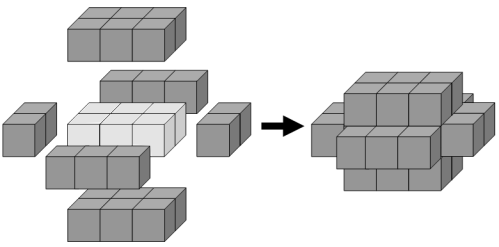
\includegraphics[width=70mm]{problems/101-200/meta/p126.png}};
    \end{tikzpicture}
\end{center}

If we then add a second layer to this solid it would require forty-six cubes to cover every visible face, the third layer would require seventy-eight cubes, and the fourth layer would require one-hundred and eighteen cubes to cover every visible face.

However, the first layer on a cuboid measuring $5 \times 1 \times 1$ also requires twenty-two cubes; similarly the first layer on cuboids measuring $5 \times 3 \times 1$, $7 \times 2 \times 1$, and $11 \times 1 \times 1$ all contain forty-six cubes.

We shall define $C(n)$ to represent the number of cuboids that contain $n$ cubes in one of its layers. So $C(22) = 2$, $C(46) = 4$, $C(78) = 5$, and $C(118) = 8$.

It turns out that $154$ is the least value of $n$ for which $C(n) = 10$.
\medskip

Find the least value of $n$ for which $C(n) = 1000$.


\section{abc-hits} \label{pb.0127}
%PB127

The radical of $n$, $rad(n)$, is the product of distinct prime factors of $n$. For example, $504 = 2^3 \times 3^2 \times 7$, so $rad(504) = 2 \times 3 \times 7 = 42$.

We shall define the triplet of positive integers $(a, b, c)$ to be an abc-hit if:

\begin{enumerate}
    \item $GCD(a, b) = GCD(a, c) = GCD(b, c) = 1$
    \item $a < b$
    \item $a + b = c$
    \item $rad(abc) < c$
\end{enumerate}
For example, (5, 27, 32) is an abc-hit, because:

\begin{enumerate}
    \item $GCD(5, 27) = GCD(5, 32) = GCD(27, 32) = 1$
    \item $5 < 27$
    \item $5 + 27 = 32$
    \item $rad(4320) = 30 < 32$
\end{enumerate}

It turns out that abc-hits are quite rare and there are only thirty-one abc-hits for $c < 1000$, with $\sum c = 12523$.

Find $\sum c$ for $c < 120000$.


\section{Hexagonal tile differences} \label{pb.0128}
%PB128

A hexagonal tile with number 1 is surrounded by a ring of six hexagonal tiles, starting at "12 o'clock" and numbering the tiles 2 to 7 in an anti-clockwise direction.

New rings are added in the same fashion, with the next rings being numbered 8 to 19, 20 to 37, 38 to 61, and so on. The diagram below shows the first three rings.

\begin{center}
    \begin{tikzpicture}
        \node[anchor=south west,inner sep=0] at (0,0) {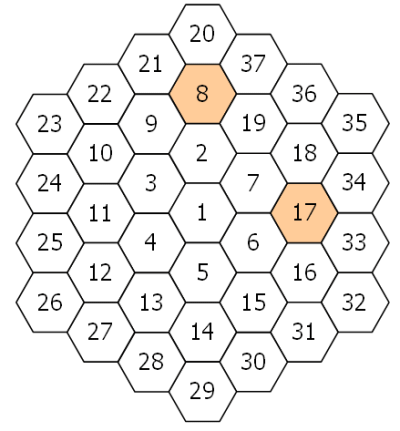
\includegraphics[width=70mm]{problems/101-200/meta/p128.png}};
    \end{tikzpicture}
\end{center}

By finding the difference between tile $n$ and each of its six neighbours we shall define $PD(n)$ to be the number of those differences which are prime.

For example, working clockwise around tile 8 the differences are $12, 29, 11, 6, 1$, and $13$. So $PD(8) = 3$.

In the same way, the differences around tile $17$ are $1, 17, 16, 1, 11,$ and $10$, hence $PD(17) = 2$.

It can be shown that the maximum value of $PD(n)$ is $3$.

If all of the tiles for which $PD(n) = 3$ are listed in ascending order to form a sequence, the $10^{\text{th}}$ tile would be $271$.

Find the $2000^{\text{th}}$ tile in this sequence.


\section{Repunit divisibility} \label{pb.0129}
%PB129

A number consisting entirely of ones is called a repunit. We shall define $R(k)$ to be a repunit of length $k$; for example, $R(6) = 111111$.

Given that $n$ is a positive integer and $GCD(n, 10) = 1$, it can be shown that there always exists a value, $k$, for which $R(k)$ is divisible by $n$, and let $A(n)$ be the least such value of $k$; for example, $A(7) = 6$ and $A(41) = 5$.

The least value of n for which A(n) first exceeds ten is 17.

Find the least value of n for which A(n) first exceeds one-million.


\section{Composites with prime repunit property} \label{pb.0130}
%PB130

A number consisting entirely of ones is called a repunit. We shall define $R(k)$ to be a repunit of length $k$; for example, $R(6) = 111111$.

Given that $n$ is a positive integer and $GCD(n, 10) = 1$, it can be shown that there always exists a value, $k$, for which R(k) is divisible by $n$, and let A(n) be the least such value of $k$; for example, $A(7) = 6$ and $A(41) = 5$.

You are given that for all primes, $p > 5$, that $p - 1$ is divisible by $A(p)$. For example, when $p = 41$, $A(41) = 5$, and $40$ is divisible by $5$.

However, there are rare composite values for which this is also true; the first five examples being $91, 259, 451, 481$, and $703$.

Find the sum of the first twenty-five composite values of $n$ for which
$GCD(n, 10) = 1$ and $n - 1$ is divisible by $A(n)$.


\section{Prime cube partnership} \label{pb.0131}
%PB131

There are some prime values, $p$, for which there exists a positive integer, $n$, such that the expression $n^3 + n^2p$ is a perfect cube.

For example, when $p = 19, 83 + 82 \times 19 = 123$.

What is perhaps most surprising is that for each prime with this property the value of $n$ is unique, and there are only four such primes below one-hundred.
\medskip

How many primes below one million have this remarkable property?


\section{Large repunit factors} \label{pb.0132}
%PB132

A number consisting entirely of ones is called a repunit. We shall define $R(k)$ to be a repunit of length $k$.

For example, $R(10) = 1111111111 = 11 \times 41 \times 271 \times 9091$, and the sum of these prime factors is $9414$.
\medskip

Find the sum of the first forty prime factors of $R(10^9)$.


\section{Repunit nonfactors} \label{pb.0133}
%PB133

A number consisting entirely of ones is called a repunit. We shall define $R(k)$ to be a repunit of length $k$; for example, $R(6) = 111111$.

Let us consider repunits of the form $R(10^n)$.

Although $R(10)$, $R(100)$, or $R(1000)$ are not divisible by $17, R(10000)$ is divisible by $17$. Yet there is no value of $n$ for which $R(10^n)$ will divide by $19$. In fact, it is remarkable that $11, 17, 41$, and $73$ are the only four primes below one-hundred that can be a factor of $R(10^n)$.
\medskip

Find the sum of all the primes below one-hundred thousand that will never be a factor of $R(10^n)$.


\section{Prime pair connection} \label{pb.0134}
%PB134


Consider the consecutive primes $p_1 = 19$ and $p_2 = 23$. It can be verified that $1219$ is the smallest number such that the last digits are formed by p1 whilst also being divisible by $p_2$.

In fact, with the exception of $p_1 = 3$ and $p_2 = 5$, for every pair of consecutive primes, $p_2 > p_1$, there exist values of $n$ for which the last digits are formed by $p_1$ and $n$ is divisible by $p_2$. Let $S$ be the smallest of these values of $n$.

Find $\sum S$ for every pair of consecutive primes with $5 \leqslant p_1 \leqslant 1000000$.


\section{Same differences} \label{pb.0135}
%PB135

Given the positive integers, $x, y$, and $z$, are consecutive terms of an arithmetic progression, the least value of the positive integer, $n$, for which the equation, $x^2 - y^2 - z^2 = n$, has exactly two solutions is $n = 27$:

$$34^2 - 27^2 - 20^2 = 12^2 - 9^2 - 6^2 = 27$$

It turns out that $n = 1155$ is the least value which has exactly ten solutions.
\medskip

How many values of $n$ less than one million have exactly ten distinct solutions?


\section{Singleton difference} \label{pb.0136}
%PB136

The positive integers, $x, y$, and $z$, are consecutive terms of an arithmetic progression. Given that $n$ is a positive integer, the equation, $x2 - y2 - z2 = n$, has exactly one solution when $n = 20$:

$$13^2 - 10^2 - 7^2 = 20$$

In fact there are twenty-five values of $n$ below one hundred for which the equation has a unique solution.
\medskip

How many values of $n$ less than fifty million have exactly one solution?



\section{Fibonacci golden nuggets} \label{pb.0137}
%PB137

Consider the infinite polynomial series $A_F(x) = xF_1 + x^2F_2 + x^3F_3 + \cdots$, where $F_k$ is the $k^{\text{th}}$ term in the Fibonacci sequence: $1, 1, 2, 3, 5, 8, ... $; that is, $F_k = F_{k-1} + F_{k-2}$, $F_1 = 1$ and $F_2 = 1$.
\medskip

For this problem we shall be interested in values of $x$ for which $A_F(x)$ is a positive integer.
\medskip

Surprisingly :

\begin{tabular}{rl}
    $A_F\left(\frac{1}{2}\right)$ & $= \left(\frac{1}{2}\right).1 + \left(\frac{1}{2}\right)^2.1 + \left(\frac{1}{2}\right)^3.2 + \left(\frac{1}{2}\right)^4.3 + \left(\frac{1}{2}\right)^5.5 + \cdots$\\
     & $= \frac{1}{2} + \frac{1}{4} + \frac{2}{8} + \frac{3}{16} + \frac{5}{32} + \cdots$\\
     & $= 2$\\
\end{tabular}
\medskip

The corresponding values of $x$ for the first five natural numbers are shown below.
\begin{center}
    \begin{tabular}{|l|c|}
        \hline
        $x$ & $A_F(x)$\\
        \hline
        $\sqrt{2}-1$ & $1$\\
        \hline
        $1/2$ & 2\\
        \hline
        $(\sqrt{13}-2)/3$ & $3$\\
        \hline
        $(\sqrt{89}-5)/8$ & $4$\\
        \hline
        $(\sqrt{34}-3)/5$ & $5$\\
        \hline
    \end{tabular}
\end{center}


We shall call $A_F(x)$ a golden nugget if $x$ is rational, because they become increasingly rarer; for example, the $10^{\text{th}}$ golden nugget is $74049690$.

Find the $15^{\text{th}}$ golden nugget.



\section{Special isosceles triangles} \label{pb.0138}
%PB138

Consider the isosceles triangle with base length, $b = 16$, and legs, $L = 17$.

\begin{center}
    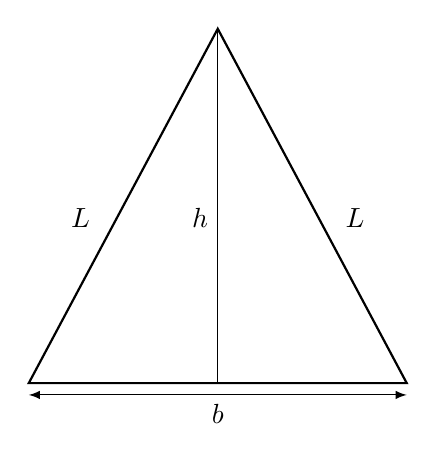
\begin{tikzpicture}[scale=0.3]
        \draw[thick] (-8,0) -- (0,15) -- (8,0) -- cycle;
        \draw (0,0) -- (0,15);
        \draw[latex-latex] (-8,-0.5) -- (8,-0.5);
        \node[below] at (0,-0.5) {$b$};
        \node[left] at (0,7) {$h$};
        \node[left] at (-5,7) {$L$};
        \node[right] at (5,7) {$L$};
        
    \end{tikzpicture}
\end{center}

By using the Pythagorean theorem it can be seen that the height of the triangle, $h = \sqrt{(17^2 - 8^2)} = 15$, which is one less than the base length.

With $b = 272$ and $L = 305$, we get $h = 273$, which is one more than the base length, and this is the second smallest isosceles triangle with the property that $h = b \pm 1$.

Find $\sum L$ for the twelve smallest isosceles triangles for which $h = b \pm 1$ and $b, L$ are positive integers.



\section{Pythagorean tiles} \label{pb.0139}
%PB139

Let $(a, b, c)$ represent the three sides of a right angle triangle with integral length sides. It is possible to place four such triangles together to form a square with length $c$.

For example, $(3, 4, 5)$ triangles can be placed together to form a $5$ by $5$ square with a $1$ by $1$ hole in the middle and it can be seen that the $5$ by $5$ square can be tiled with twenty-five 1 by 1 squares.

\begin{center}
    \begin{tikzpicture}[scale=1]
        \draw(0,0) -- (0,5) -- (5,5) -- (5,0) -- cycle;
        \draw (0,1) -- (5,1)  (0,2) -- (5,2)  (0,3) -- (5,3)  (0,4) -- (5,4)  (1,0) -- (1,5)  (2,0) -- (2,5)  (3,0) -- (3,5)  (4,0) -- (4,5);
        
        \draw (-6,0) -- (-6,5) -- (-1,5) -- (-1,0) -- cycle;
    \end{tikzpicture}
\end{center}

However, if $(5, 12, 13)$ triangles were used then the hole would measure $7$ by $7$ and these could not be used to tile the $13$ by $13$ square.

Given that the perimeter of the right triangle is less than one-hundred million, how many Pythagorean triangles would allow such a tiling to take place?


\section{Modified Fibonacci golden nuggets} \label{pb.0140}
%PB140

Consider the infinite polynomial series $A_G(x) = xG_1 + x^2G_2 + x^3G_3 + \cdots,$ where Gk is the $k^{\text{th}}$ term of the second order recurrence relation $G_k = G_{k-1} + G_{k-2}$, $G_1 = 1$ and $G_2 = 4$; that is, $1, 4, 5, 9, 14, 23, ...$ .


For this problem we shall be concerned with values of $x$ for which $A_G(x)$ is a positive integer.

The corresponding values of $x$ for the first five natural numbers are shown below.

\begin{center}
    \begin{tabular}{|l|c|}
        \hline
        $x$ & $A_G(x)$\\
        \hline
        $(\sqrt{5}-1)/4$ & $1$\\
        \hline
        $2/5$ & $2$\\
        \hline
        $(\sqrt{22}-2)/6$ & $3$\\
        \hline
        $(\sqrt{137}-5)/14$ & $4$\\
        \hline
        $1/2$ & $5$\\
        \hline
    \end{tabular}
\end{center}

We shall call $A_G(x)$ a golden nugget if $x$ is rational, because they become increasingly rarer; for example, the $20^{\text{th}}$ golden nugget is 211345365.

Find the sum of the first thirty golden nuggets.


\section{Investigating progressive numbers, $n$, which are also square} \label{pb.0141}
%PB141

A positive integer, n, is divided by d and the quotient and remainder are q and r respectively. In addition d, q, and r are consecutive positive integer terms in a geometric sequence, but not necessarily in that order.

For example, 58 divided by 6 has quotient 9 and remainder 4. It can also be seen that 4, 6, 9 are consecutive terms in a geometric sequence (common ratio 3/2).
We will call such numbers, n, progressive.

Some progressive numbers, such as 9 and 10404 = 1022, happen to also be perfect squares.
The sum of all progressive perfect squares below one hundred thousand is 124657.

Find the sum of all progressive perfect squares below one trillion $(10^12)$.


\section{} \label{pb.0142}
%PB142


\section{} \label{pb.0143}
%PB143


\section{} \label{pb.0144}
%PB144


\section{} \label{pb.0145}
%PB145


\section{} \label{pb.0146}
%PB146


\section{} \label{pb.0147}
%PB147


\section{} \label{pb.0148}
%PB148


\section{} \label{pb.0149}
%PB149


\section{} \label{pb.0150}
%PB150


